\chapter{Foundational implementations}\label{chap:libs}

This chapter presents the rationale behind our choice of QUIC and MQTT implementations.
In terms of QUIC, we used the $quinn$ implementation in order to create the intermediate library discussed in Chapter~\ref{chapter:quic_socket}.
On the MQTT side, $rumqtt$ was used as the starting point for our MQTT/QUIC implementation.

The choice criteria follow from the previously presented background and some general criteria.
We analysed the available implementations based on their storage footprint, the programming language they were implemented in, their use of TLS, widespread adoption and availability of documentation.

\subsection{QUIC} \label{section:quic_impl}

We now compare the existing implementations of the QUIC protocol in the context of usability for IoT devices and present the reasoning behind our choice of QUIC library.
We have considered the mainstream implementations in the C, C++, Rust and Go programming languages as these are the languages that can be considered systems languages and would thus be the most widely used ones for IoT devices.
In addition to this, we did not consider implementations paired with a browser web engine as these would be impossible to use on hardware constrained devices.
Hence, we did not include notable implementations such as the QUIC implementation of the chromium web engine~\citep{chromium_quic_2021} and $Neqo$~\citep{mozilla_neqo_2022}.

Importantly, to analyse the performance of underlying QUIC implementations, we have transferred the same file using each implementation several times and have taken the average time to do so.
We repeated this while altering parameters as described in Section~\ref{chap:net_sim}.
The differences in transfer time were negligible and have hence not been presented as part of the comparison of libraries.
Hence, we compare QUIC implementations in terms of their TLS use, programming language and the binary size produced by their client and server implementations.

First, we consider the general landscape of available QUIC implementations to contextualise the ones developed in Rust.
Table~\ref{tab:quics} demonstrates the analysed QUIC implementations.
In order to find the size of the binary, we have used the Linux $ls$ utility.
In the case of the $mvfst$ implementation, we have taken further steps due to the reported binary size being far too large.
Therefore, we had to remove the C++ debug symbols that were causing the binary size to be over 300 MiB.
We have identified the following main methods by which QUIC implementations incorporate TLS:

\begin{itemize}
    \item Use of an external library - the implementation uses an external TLS API either by using a package manager in the case of Rust or by relying on an installed implementation in the case of C and C++.
    \item Use of own implementation - the implementation packages its implementation of the TLS protocol alongside QUIC.
\end{itemize}

This different use of TLS presented a challenge in calculating the binary size of the QUIC servers and clients.

\begin{table}[ht]
    \caption{The identified QUIC implementations and their binary size footprint. The footprint has been split into a client and server footprint using a minimal reproducible example for each. We used each implementation to create an example client and server capable of sending and receiving QUIC packets and analysed the binary size. Where provided, we compared this to the given examples to ensure as little implementation bias as possible. However, this is still not a perfect estimate, and some variance due to implementation details may be present.}\label{tab:quics}
    %\tt 
    \rowcolors{2}{}{gray!3}
    \begin{tabular}{@{}lllll@{}}
        \toprule
        \textbf{Implementation} & \textbf{PL}   & \textbf{Footprint (client) (MiB)} & \textbf{Footprint (server) (MiB)} & \textbf{TLS method} \\
        ngtcp2                  & \texttt{C}    & \texttt{3.4}                      & \texttt{4.3}                      & \texttt{External}   \\
        picoquic                & \texttt{C}    & \texttt{3.2}                      & \texttt{3.9}                      & \texttt{External}   \\
        msquic                  & \texttt{C}    & \texttt{3.2}                      & \texttt{4.1}                      & \texttt{External}   \\
        quic-go                 & \texttt{Go}   & \texttt{8.7}                      & \texttt{9.9}                      & \texttt{External}   \\
        Quinn                   & \texttt{Rust} & \texttt{9.1}                      & \texttt{9.5}                      & \texttt{External}   \\
        Quiche                  & \texttt{Rust} & \texttt{7.8}                      & \texttt{7.0}                      & \texttt{Own}        \\
        mvfst                   & \texttt{C++}  & \texttt{11.1}                     & \texttt{12.0}                     & \texttt{Own}        \\
        \bottomrule
    \end{tabular}
\end{table}

Specifically, in each case, we have considered the external dependencies that a developer will have to install to run the QUIC implementation on a device.
Hence, in the case of C implementations that require an external TLS library, such as OpenSSL, to be installed and linked on the system, we have opted to add the binary size produced by OpenSSL to the size of the QUIC binaries.
Additionally, in the case of $picoquic$, we have added the size of the $picotls$ dependency on top of the size of OpenSSL.

\begin{figure}[ht]
    \centering
    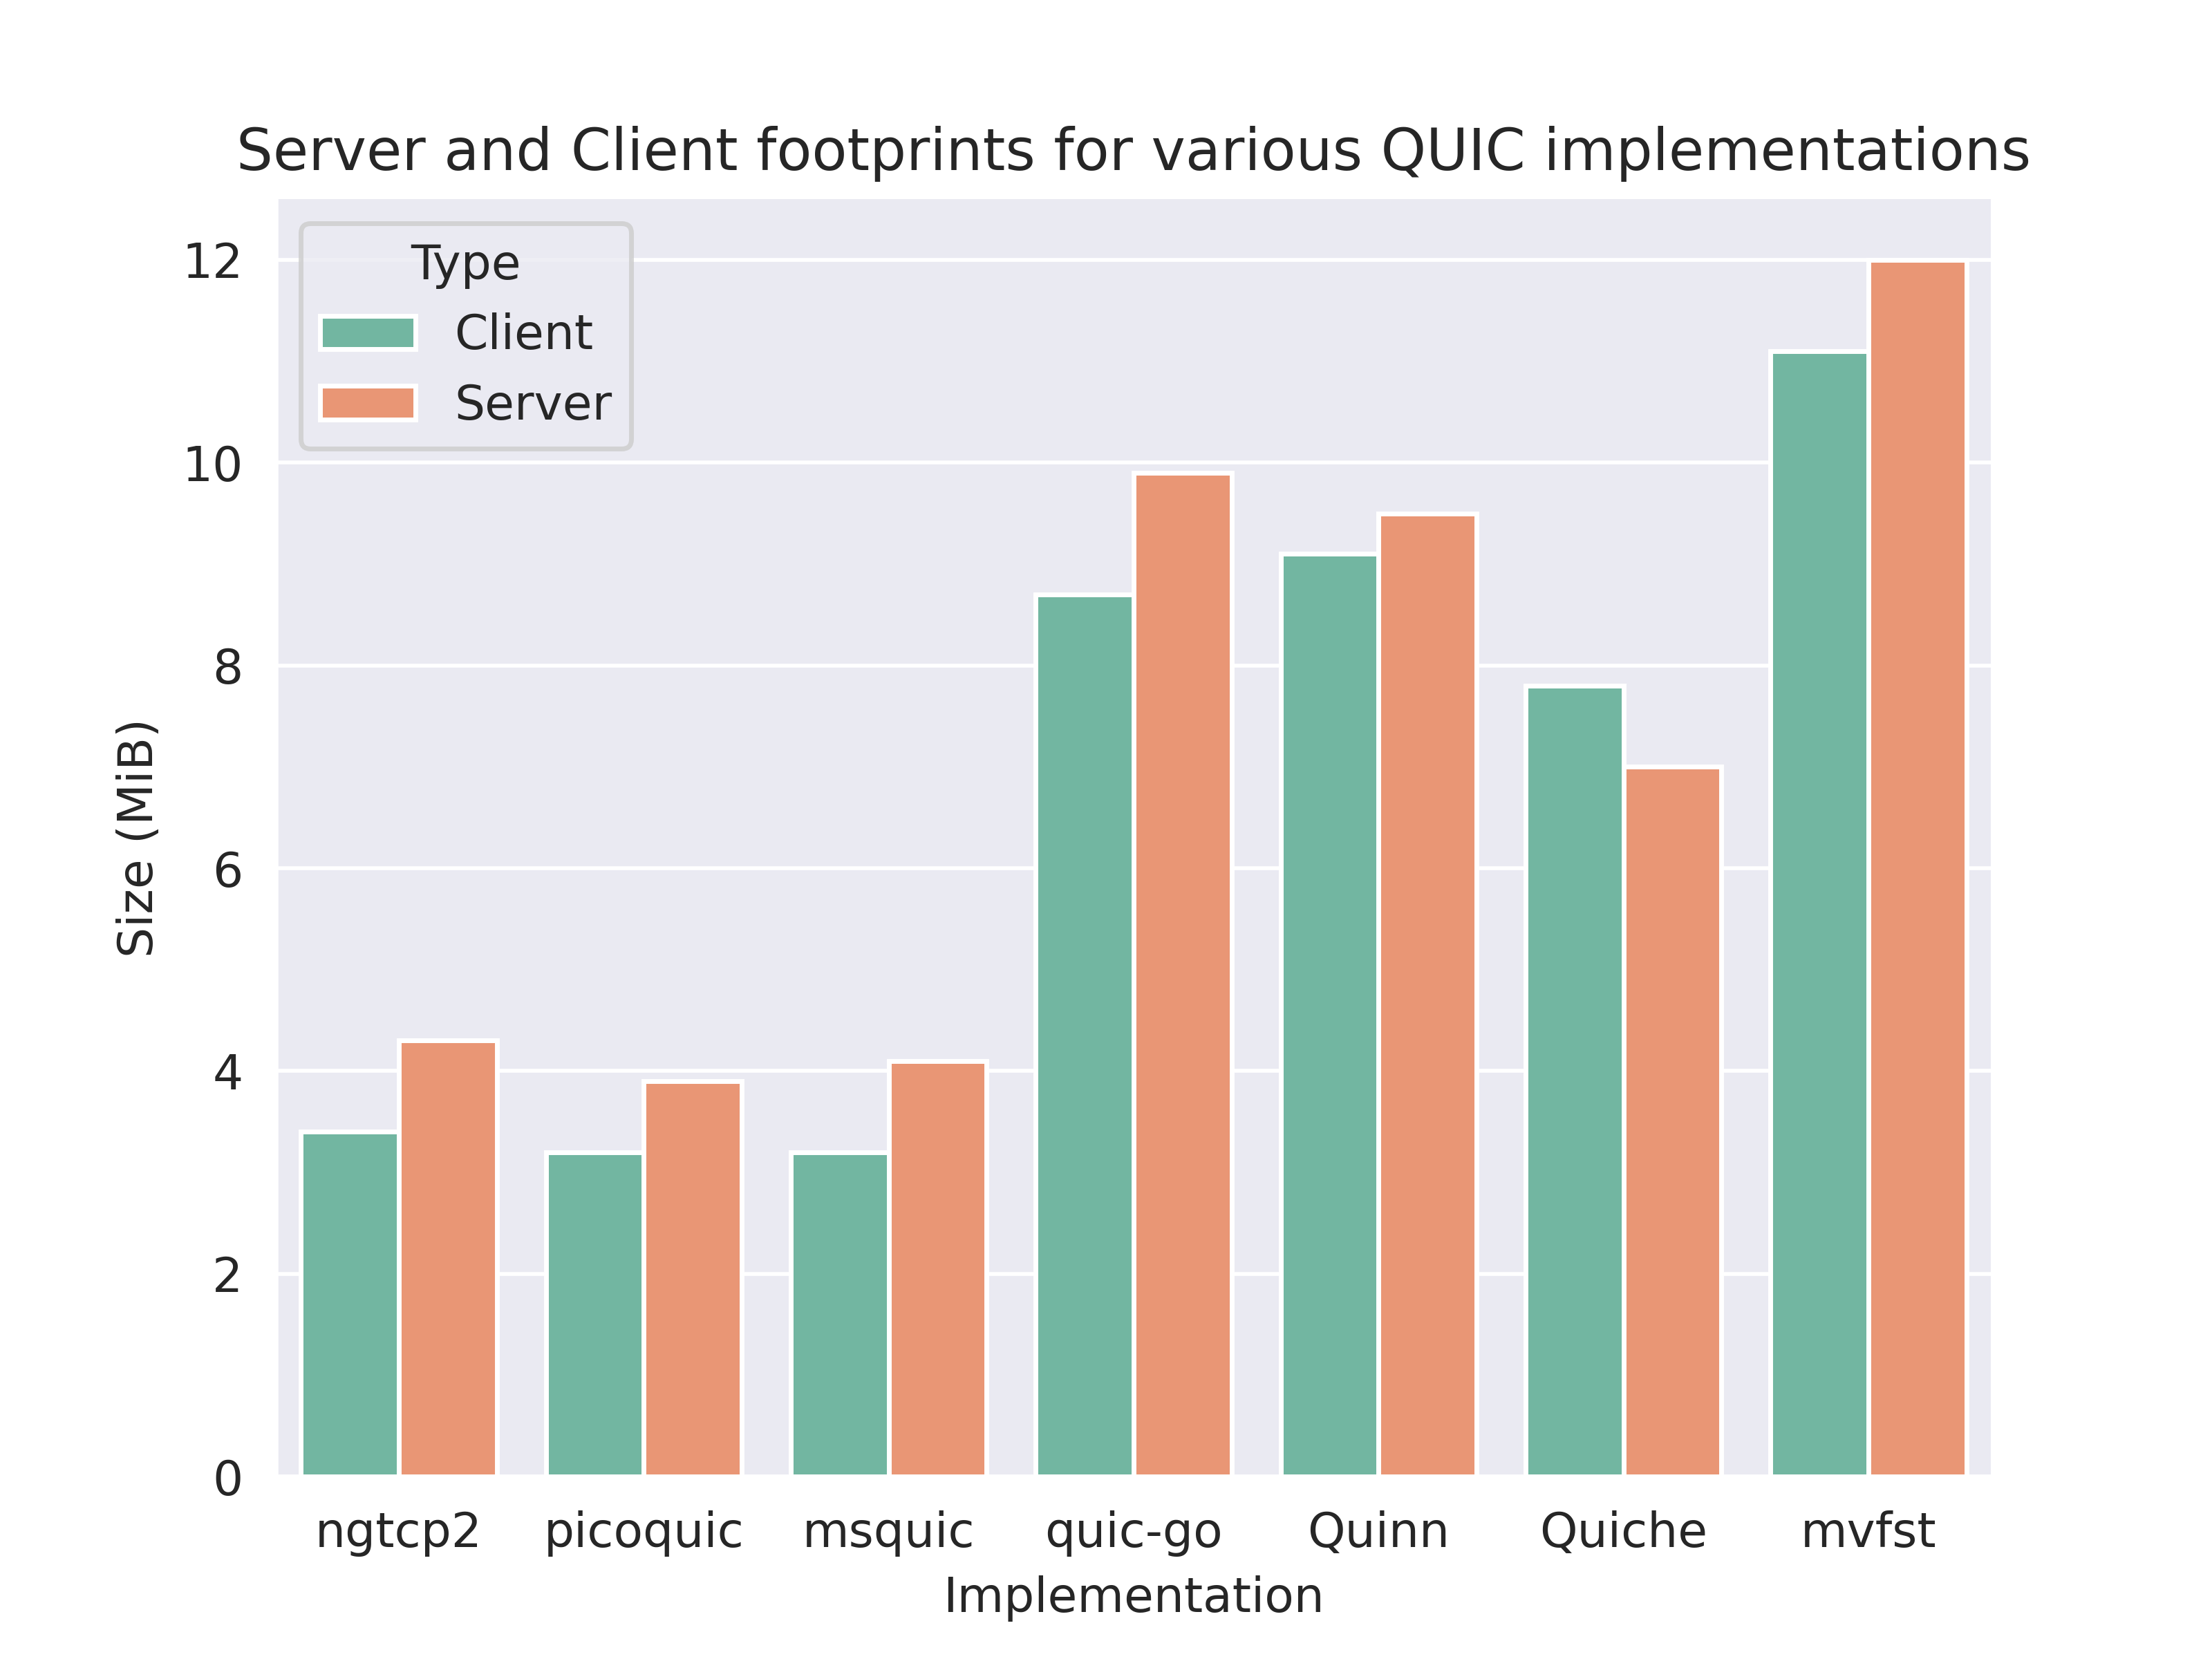
\includegraphics[width=1\linewidth]{images/quic_impls.png}
    \caption{The sizes of the client and server footprints for the selected QUIC implementations. Notable, only Quiche produced a server binary with a smaller size than its corresponding client binary. It is hard to estimate the error margin for the data as this depends on implementation details in the example client and servers.}
    \label{fig:quic_impls}
\end{figure}

Figure~\ref{fig:quic_impls} further visualises the comparison of binary sizes between the various implementations.
This is an important aspect due to the aforementioned hardware constraints.
Notably, we can see that five out of the seven analysed implementations opt to use an external TLS library or engine.
Out of these five, all C implementations supported OpenSSL, with the Go and Rust implementations opting to use a TLS library.
In the case of $quic-go$, this was the $crypto/tls$ package, and in the case of Rust, $rustls$.
We can also see that the Rust implementations are not drastically different in binary footprint size.

Notably, although Go is described as memory safe, it does not opt for compile-time memory safety and instead uses the panic model.
The panic model is another advantage of Rust compared to languages such as Go, as Rust provides these guarantees using a robust type system.
Between the two Rust implementations - Quinn and Quiche, we chose Quinn due to issues with the Quiche library.
On the other hand, Quiche opts to make the user create a $mio$ event loop, which interfered with the $tokio$ runtime environment used in our chosen MQTT implementation discussed in the next section.
In addition to this, we found that the Quinn API is easier to work with when creating the intermediate library discussed in Chapter~\ref{chapter:quic_socket}; for example, Quinn handles the QUIC handshake in the library and does not require the developer to create an event loop.

\section{MQTT}\label{section:mqtt_impls}

Compared to QUIC, the choice of MQTT implementation was substantially simpler.
The criteria for MQTT implementation were that it was developed in Rust, implemented both a client and a broker, had widespread use and adhered to MQTT version 5.0.
Based on the above criteria we identified two possible implementations:\citepos{eclipse_eclipse_2018} $paho$ and $rumqtt$~\citep{bytebeam_rumqtt_2020}.
We opted to use $rumqtt$ at it is a native Rust implementation, whereas $paho$ provides a rust binding to an underlying C implementation.
We chose to evaluate a fully Rust native MQTT/QUIC stack as this provides an opportunity for a valuable comparison to mainstream C implementations.
Other available implementations supported only one side of the MQTT protocol or only supported version 3.1.1.

$Rumqtt$ provides to components for an MQTT application - $rumqttc$ and $rumqttd$.
The former can be used to create an MQTT client, and the latter a broker.
However, the code base for these is somewhat similar, easing the incorporation of QUIC.
Both components provide an interface for supporting asynchronous communication using a $tokio$ runtime, which fits nicely into our choice of QUIC implementation as $Quinn$ requires a $tokio$ environment.
By default, $rumqtt$ uses TCP as its transport layer protocol and TLS through $rustls$.
All underlying implementation assumptions remain equal because this is the same library as $Quinn$ uses.
